\clearpage
\section{A concrete experimental protocol}
\label{sec:protocol}
\subsection{Establish three separate levels of evidence}
\begin{figure}[!ht]
\centering
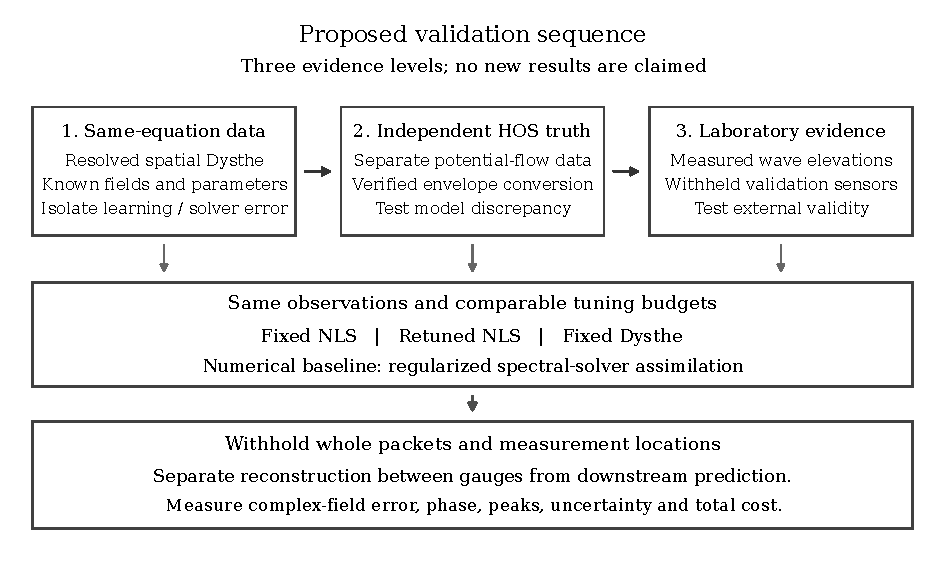
\includegraphics[width=\textwidth]{figures/experiment-design.pdf}
\caption{Proposed study design. Same-equation synthetic tests establish
implementation accuracy; independently generated HOS and laboratory data
address different model-validity questions. These levels must keep their
original physical provenance. The diagram contains no experimental results.}
\label{fig:design}
\end{figure}

\begin{enumerate}
\item \textbf{Numerical accuracy for the declared equation.}
Use plane waves and the mathematical NLS control for elementary checks,
then converged Dysthe packet trajectories. Independently refine
propagation step, profile resolution, nonlinear quadrature, and domain
length. Agreement with one's own unresolved training data is insufficient.
\item \textbf{Approximation of more complete water-wave physics.}
Use HOS truth with its original model label and a documented envelope
extraction map. The public dataset \cite{hosdata} is a candidate source,
not automatically a Dysthe benchmark. Select compatible unidirectional,
deep-water, narrowband cases and justify the validity bounds.
\item \textbf{Measurement performance.}
Use laboratory observations with calibration and noise information.
Assess only quantities independently observed or otherwise supported.
Reconstructing an unmeasured latent potential is not its experimental
validation. Do not make operational sea-state claims from tank data alone.
\end{enumerate}

\subsection{Minimal pilot before a large campaign}
The following is a proposed workload, not an existing result or a universal
sample-size requirement. Begin with three regimes spanning low to moderate
steepness/bandwidth within justified limits, two gauge separations, two
noise levels, and five independently drawn packets per cell:
$3\times2\times2\times5=60$ inverse cases. The noise-free level checks
implementation; the other should reflect an explicit sensor-noise model.
Choose physical parameter values only after reference-resolution and
envelope-validity checks. The $60$ cases are for feasibility, not enough
by themselves to settle all regime interactions.

Run the three equation arms and two inference engines of Question 1.
Start with a few optimizer seeds on the pilot, then choose replication
from observed variability. For the final comparison, use paired initial
fields and noise realizations, report median and upper-tail errors, and
bootstrap whole trajectories rather than individual grid points.
Record optimization failures; do not discard them from the success rate.
A larger study can use a space-filling design followed by targeted
sampling near changes in the relative model performance.

\subsection{A practical PINN starting recipe}
The following is a proposed baseline assembled from inspected methods;
its Dysthe performance remains to be established.
\begin{enumerate}
\item \textbf{Scale the problem.}
Use the recorded physical normalization, nondimensional coordinates,
and training-only feature scaling. Start with double precision for
reference and residual qualification, then measure whether reduced
precision preserves the required accuracy.
\item \textbf{Represent periodicity correctly.}
For an exact periodic inlet $u_0$, use commensurate features such as
$\cos(2\pi\tau/L),\sin(2\pi\tau/L)$ and an ansatz
\[
 u_\theta(\xi,\tau)=u_0(\tau)
       +\frac{\xi}{\Xi}N_\theta\!\left(
          \frac{\xi}{\Xi},\cos(2\pi\tau/L),\sin(2\pi\tau/L)\right),
 \quad 0\leq\xi\leq\Xi .
\]
This enforces the initial field and periodic profile by construction.
If $u_0$ is uncertain, infer a latent inlet and penalize its disagreement
with measurements according to the noise model instead of hard-coding
noisy observations. Random Fourier frequencies are not automatically
periodic with period $L$.
\item \textbf{Evaluate the nonlocal term on complete slices.}
Evaluate the field on a uniform periodic profile grid at sampled
$\xi$ values, apply a differentiable FFT multiplier, and evaluate
products using justified anti-aliasing/projection choices. Validate the
result independently on a finer grid. Record that the residual contains
a numerical spectral operator.
\item \textbf{Use a credible optimizer comparison.}
Compare an Adam-to-L-BFGS recipe with self-scaled Broyden and, if resources
permit, SOAP. Resampling changes the optimization objective and may
interact with quasi-Newton history; specify when points are frozen or
history is reset. Count line searches and derivative evaluations.
\item \textbf{Add complexity one ingredient at a time.}
After the basic model works, test $\xi$ slabs/causal weights, complex
layers, adaptive sampling, and appropriate invariant penalties. Tune
each on validation cases. A large combination without ablations does
not explain why a method works.
\end{enumerate}

\subsection{Metrics that match the scientific claim}
Let $u$ denote a resolved reference and $\widehat u$ a prediction on a
fixed evaluation domain $\Omega$, with physical quadrature weights.
Report at least
\begin{align}
 E_{\rm field}&=\frac{\norm{\widehat u-u}_{L^2(\Omega)}}
                         {\norm{u}_{L^2(\Omega)}},&
 E_{\rm amp}&=\frac{\norm{|\widehat u|-|u|}_{L^2(\Omega)}}
                         {\norm{u}_{L^2(\Omega)}}. \label{eq:metrics}
\end{align}
For meaningful phase evaluation define
$A_\eta=\{(\xi,\tau):|u|\geq\eta,\ |\widehat u|\geq\eta\}$
using a documented amplitude threshold and use, for example,
\[
 E_\phi^2=
 \frac{\int_{A_\eta}|u|^2
     \Arg(\widehat u\,\overline u)^2\dd\xi\dd\tau}
      {\int_{A_\eta}|u|^2\dd\xi\dd\tau}.
\]
If the denominator vanishes, report the metric as undefined. Also report
the fraction of the domain retained by the threshold. Phase- or
translation-aligned errors can diagnose mistakes, but must be accompanied
by unaligned errors and the fitted shifts.

Additional measurements should include:
\begin{itemize}
\item envelope peak height, focusing distance, retarded-time location,
and event detection precision/recall at preregistered thresholds;
\item profile spectra and spectral-edge content; correct invariant
defects, interpreted alongside reference discretization error;
\item withheld surface-elevation error after a fixed observation map;
SSP may aid comparison with water-wave papers but is not interchangeable
with complex-field relative $L^2$ error;
\item coefficient recovery and calibrated interval coverage when
parameters are actually identifiable;
\item training, tuning, data-generation, adaptation and inference time,
peak memory, and total residual/operator evaluations.
\end{itemize}
Never label a small invariant defect, a low training loss, or a visually
plausible envelope an accuracy certificate.

\subsection{Fair comparisons and explicit decision gates}
Separate a best-accuracy experiment from a fixed-budget experiment.
Allow comparable hyperparameter-selection resources, keep the final
test set untouched, and disclose hardware and numerical precision.
Charge adaptive candidate scoring and sampler maintenance
\cite{operatorbudget}; iteration counts alone can hide significant costs.

Before the final campaign, choose a minimum practically useful improvement
and tolerable cost ratio. For example, a \emph{proposed} pilot continuation
rule could require a $20\%$ reduction in median held-out phase or
field error, a paired confidence interval excluding no improvement, and
no material degradation in upper-tail event error. This number is a
project decision to be justified, not a literature standard. If the
reference uncertainty is comparable to the claimed improvement, tighten
the reference first. If no practically useful gain appears, simplify
the method or redirect to the documented identifiability limitation.

\clearpage
\section{Roadmap, current assets, and delivery limits}
\subsection{A staged route to a submission}
The schedule below is an indicative planning estimate, conditional on
compute, data access, and successful validation.
\begin{longtable}{@{}P{0.15\textwidth}P{0.43\textwidth}P{0.34\textwidth}@{}}
\toprule
Stage & Deliverable & Gate before proceeding \\
\midrule
\endfirsthead
\toprule
Stage & Deliverable & Gate before proceeding \\
\midrule
\endhead
Weeks 1--2 & Reproduce one direct NLS baseline; verify the exact
Dysthe residual and observation conversion. & Correct signs, mean flow,
boundary conditions, and independent refinement evidence. \\
Weeks 3--4 & Numerical assimilation and modern PINN pilot;
local sensitivity/identifiability analysis. & Equal observations and
credible simpler-model controls; meaningful effect size. \\
Weeks 5--7 & Expand regimes, seeds, and held-out packets;
one targeted ablation from Question 3. & Stable gains or a robust,
explainable failure boundary. \\
Weeks 8--10 & External HOS or laboratory validation; uncertainty
and cost evaluation; manuscript and reproducibility package. &
Claims match the actual evidence level and survive negative controls. \\
Later & Operator amortization or rigorous certification. &
Strong first-stage baselines; separate novelty and feasibility review. \\
\bottomrule
\end{longtable}

Do not begin all five questions simultaneously. Question 1 with a focused
part of Question 2 supplies a coherent first manuscript. Question 3 can
provide a method explanation if the pilot identifies a genuine training
bottleneck. Question 4 becomes sensible only when repeated-query demand
and dataset costs are known; Question 5 is a separate mathematical track.

\subsection{What is available locally now}
Read-only inspection of the current family confirmed the model contract
and an implemented \texttt{SpatialDysthe} reference solver in
\path{dysthe-core/src/dysthe_core/reference/spatial.py}.
The equation specification is
\path{dysthe-core/docs/model.md}; qualification guidance is
\path{dysthe-core/docs/stage-one-reference.md}.
The FNO and hybrid method READMEs in \texttt{dysthe-learning} still describe
planned methods. This is a current file inspection, not a fresh numerical
qualification or training result. Historical artifacts must retain their
actual equation labels.

The current solver is therefore a starting asset to qualify, rather than
a reason to build an unrelated simulator. The paper should use
\texttt{dysthe-experiments} for frozen campaigns and splits,
\texttt{dysthe-learning} for compared methods, and
\texttt{dysthe-paper} for numerical evidence once experiments exist.
This review does not modify those implementations or assert that the
proposed experiments have been completed.

\subsection{Verification and limitations of this review}
This report provides live primary-source literature checking, access and
status distinctions, explicit future-work provenance, an independent
check of the elementary NLS example and estimate, and original vector
figures. Several very recent Elsevier/Springer papers were accessible
only through abstracts and previews; their full comparative claims,
code, and statistical evidence could not be audited. The stronger
full-text sources and those preview-only leads are identified separately.

No literature experiment, public training code, HOS dataset, or local
solver qualification campaign was rerun. No definitive claim of novelty,
universal best method, ocean-operational readiness, or established
Dysthe--PINN advantage is made. The main deliverable is a concrete,
testable research program grounded in the verified sources below.
